\documentclass{beamer}

\pdfmapfile{+sansmathaccent.map}


\mode<presentation>
{
	\usetheme{Warsaw} % or try Darmstadt, Madrid, Warsaw, Rochester, CambridgeUS, ...
	\usecolortheme{seahorse} % or try seahorse, beaver, crane, wolverine, ...
	\usefonttheme{serif}  % or try serif, structurebold, ...
	\setbeamertemplate{navigation symbols}{}
	\setbeamertemplate{caption}[numbered]
} 


%%%%%%%%%%%%%%%%%%%%%%%%%%%%
% itemize settings

\definecolor{myhotpink}{RGB}{255, 80, 200}
\definecolor{mywarmpink}{RGB}{255, 60, 160}
\definecolor{mylightpink}{RGB}{255, 80, 200}
\definecolor{mypink}{RGB}{255, 30, 80}
\definecolor{mydarkpink}{RGB}{155, 25, 60}

\definecolor{mypaleblue}{RGB}{240, 240, 255}
\definecolor{mylightblue}{RGB}{120, 150, 255}
\definecolor{myblue}{RGB}{90, 90, 255}
\definecolor{mygblue}{RGB}{70, 110, 240}
\definecolor{mydarkblue}{RGB}{0, 0, 180}
\definecolor{myblackblue}{RGB}{40, 40, 120}

\definecolor{mygreen}{RGB}{0, 200, 0}
\definecolor{mygreen2}{RGB}{245, 255, 230}

\definecolor{mygray}{gray}{0.8}
\definecolor{mydarkgray}{RGB}{80, 80, 160}

\definecolor{mydarkred}{RGB}{160, 30, 30}
\definecolor{mylightred}{RGB}{255, 150, 150}
\definecolor{myred}{RGB}{200, 110, 110}
\definecolor{myblackred}{RGB}{120, 40, 40}

\definecolor{mygreen}{RGB}{0, 200, 0}
\definecolor{mygreen2}{RGB}{205, 255, 200}

\definecolor{mydarkcolor}{RGB}{60, 25, 155}
\definecolor{mylightcolor}{RGB}{130, 180, 250}

\setbeamertemplate{itemize items}[default]

\setbeamertemplate{itemize item}{\color{myblackblue}$\blacksquare$}
\setbeamertemplate{itemize subitem}{\color{mydarkblue}$\blacktriangleright$}
\setbeamertemplate{itemize subsubitem}{\color{mygray}$\blacksquare$}

\setbeamercolor{palette quaternary}{fg=white,bg=mygblue} %mydarkgray
\setbeamercolor{titlelike}{parent=palette quaternary}

\setbeamercolor{palette quaternary2}{fg=white,bg=mygblue}%black myblue
\setbeamercolor{frametitle}{parent=palette quaternary2}

\setbeamerfont{frametitle}{size=\Large,series=\scshape}
\setbeamerfont{framesubtitle}{size=\normalsize,series=\upshape}


%%%%%%%%%%%%%%%%%%%%%%%%%%%%
% block settings

%\setbeamercolor{block title}{bg=red!50,fg=black}
%\setbeamercolor{block title}{bg=mylightblue,fg=black}
\setbeamercolor{block title}{bg=myblackblue,fg=white}

\setbeamercolor*{block title example}{bg=mygreen!40!white,fg=black}

\setbeamercolor*{block body example}{fg= black,
	bg= mygreen2}


%%%%%%%%%%%%%%%%%%%%%%%%%%%%
% URL settings
\hypersetup{
	colorlinks=false,
	linkcolor=blue,
	filecolor=blue,      
	urlcolor=blue,
}

%%%%%%%%%%%%%%%%%%%%%%%%%%

\renewcommand{\familydefault}{\rmdefault}

\usepackage{amsmath}
\usepackage{mathtools}

\usepackage{subcaption}

\usepackage{qrcode}

\DeclareMathOperator*{\argmin}{arg\,min}
\newcommand{\bo}[1] {\mathbf{#1}}

\newcommand{\dx}[1] {\dot{\mathbf{#1}}}
\newcommand{\ma}[4] {\begin{bmatrix}
		#1 & #2 \\ #3 & #4
\end{bmatrix}}
\newcommand{\myvec}[2] {\begin{bmatrix}
		#1 \\ #2
\end{bmatrix}}
\newcommand{\myvecT}[2] {\begin{bmatrix}
		#1 & #2
\end{bmatrix}}

\newcommand{\R}{\mathbb{R}} 
\newcommand{\T}{^\top}     



\newcommand{\mydate}{Spring 2023}

\newcommand{\mygit}{\textcolor{blue}{\href{https://github.com/SergeiSa/Computational-Intelligence-Slides-Spring-2023}{github.com/SergeiSa/Computational-Intelligence-Slides-Spring-2023}}}

\newcommand{\myqr}{ \textcolor{black}{\qrcode[height=1.5in]{https://github.com/SergeiSa/Computational-Intelligence-Slides-Spring-2023}}
}

\newcommand{\myqrframe}{
	\begin{frame}
		\centerline{Lecture slides are available via Github, links are on Moodle}
		\bigskip
		\centerline{You can help improve these slides at:}
		\centerline{\mygit}
		\bigskip
		\myqr
	\end{frame}
}


\newcommand{\bref}[2] {\textcolor{blue}{\href{#1}{#2}}}



%%%%%%%%%%%%%%%%%%%%%%%%%%%%
% code settings

\usepackage{listings}
\usepackage{color}
% \definecolor{mygreen}{rgb}{0,0.6,0}
% \definecolor{mygray}{rgb}{0.5,0.5,0.5}
\definecolor{mymauve}{rgb}{0.58,0,0.82}
\lstset{ 
	backgroundcolor=\color{white},   % choose the background color; you must add \usepackage{color} or \usepackage{xcolor}; should come as last argument
	basicstyle=\footnotesize,        % the size of the fonts that are used for the code
	breakatwhitespace=false,         % sets if automatic breaks should only happen at whitespace
	breaklines=true,                 % sets automatic line breaking
	captionpos=b,                    % sets the caption-position to bottom
	commentstyle=\color{mygreen},    % comment style
	deletekeywords={...},            % if you want to delete keywords from the given language
	escapeinside={\%*}{*)},          % if you want to add LaTeX within your code
	extendedchars=true,              % lets you use non-ASCII characters; for 8-bits encodings only, does not work with UTF-8
	firstnumber=0000,                % start line enumeration with line 0000
	frame=single,	                   % adds a frame around the code
	keepspaces=true,                 % keeps spaces in text, useful for keeping indentation of code (possibly needs columns=flexible)
	keywordstyle=\color{blue},       % keyword style
	language=Octave,                 % the language of the code
	morekeywords={*,...},            % if you want to add more keywords to the set
	numbers=left,                    % where to put the line-numbers; possible values are (none, left, right)
	numbersep=5pt,                   % how far the line-numbers are from the code
	numberstyle=\tiny\color{mygray}, % the style that is used for the line-numbers
	rulecolor=\color{black},         % if not set, the frame-color may be changed on line-breaks within not-black text (e.g. comments (green here))
	showspaces=false,                % show spaces everywhere adding particular underscores; it overrides 'showstringspaces'
	showstringspaces=false,          % underline spaces within strings only
	showtabs=false,                  % show tabs within strings adding particular underscores
	stepnumber=2,                    % the step between two line-numbers. If it's 1, each line will be numbered
	stringstyle=\color{mymauve},     % string literal style
	tabsize=2,	                   % sets default tabsize to 2 spaces
	title=\lstname                   % show the filename of files included with \lstinputlisting; also try caption instead of title
}

%%%%%%%%%%%%%%%%%%%%%%%%%%%%
% tikz settings

\usepackage{tikz}
\tikzset{every picture/.style={line width=0.75pt}}

%%%%%%%%%%%%%%%%%%%%%%%%%%%%




\title{Shortest Path Planning}
\subtitle{Computational Intelligence, Lecture 13}
\author{by Sergei Savin}
\centering
\date{\mydate}


\begin{document}
\maketitle


\begin{frame}{Content}

%\begin{itemize}
%\item Mixed Integer Linear Programming (MILP)
%\item Mixed Integer Quadratic Programming (MIQP)
%\item Example: Footstep planning
%\item Big-M method relaxation
%\item Example: switching control
%\item Homework
%\end{itemize}

\end{frame}



\begin{frame}{Shortest path on a graph}
	%\framesubtitle{General form}
	\begin{flushleft}
		
		If we want to plan a path on a 2D map, we can represent obstacle-free space regions as a nodes, and possible transitions between the obstacle-free space regions as graph edges. 
		
		\begin{figure}
			\centering
			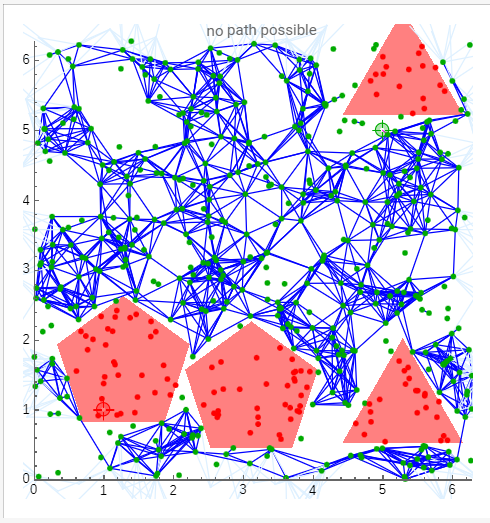
\includegraphics[width=0.4\linewidth]{GraphPathPlanning}
			\caption{Path planning as graph search; \scriptsize{Credit: https://demonstrations.wolfram.com/ProbabilisticRoadmapMethod/}}
			\label{fig:graphpathplanning}
		\end{figure}
		
		
	\end{flushleft}
\end{frame}



\begin{frame}{Shortest path on a graph}
%\framesubtitle{General form}
\begin{flushleft}

Consider a directed graph (each edge has a direction assigned to it):

% TODO: \usepackage{graphicx} required
\begin{figure}
	\centering
	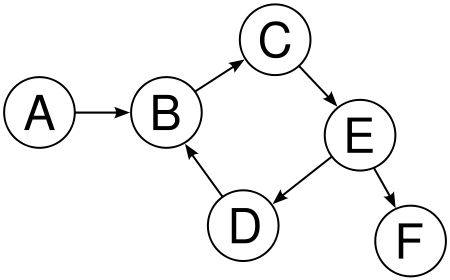
\includegraphics[width=0.5\linewidth]{DirectedGraph}
	\caption[]{Directed graph; \scriptsize{Credit: https://github.com/HQarroum/directed-graph}}
	\label{fig:directedgraph}
\end{figure}

How can we find a shortest path from a start node to a finish node on it?

\end{flushleft}
\end{frame}

\begin{frame}
	%\framesubtitle{How do we know the state?}
	\begin{flushleft}
		
		\centering{\Huge SPP as LP}
		
	\end{flushleft}
\end{frame}

\begin{frame}{Shortest path (1)}
%\framesubtitle{General form}
\begin{flushleft}

We assign index variable $x_i$ to $i$-th edge; each index variable is positive $x_i \geq 0$. 

\bigskip

If $x_i = 1$ the edge is part of the path. We assume that otherwise $x_i = 0$ (which will be enforced by the other constraints). Adding a cost $d_i$ associated with each edge (e.g. Euclidean distance) we get a linear cost $l(\bo{x})$:

\begin{equation}
	l(\bo{x}) = \bo{x}\T \bo{d}
\end{equation}

 
\end{flushleft}
\end{frame}



\begin{frame}{Shortest path (2)}
	%\framesubtitle{General form}
	\begin{flushleft}
		
		Since each edge connects one node (e.g. node $u$) to another (e.g. node $v$), we can label all index variables $x$ with superscripts, denoting nodes that they connect - $x^{u,v}$.
		
		\bigskip
		
		Our goal will be to count how many path segments enter and leave each node. For any normal node the number will be equal:
		
		\begin{equation}
			-\sum_{\forall i} x^{i,v} + \sum_{\forall j} x^{v,j} = 0
		\end{equation}
		
	
	\end{flushleft}
\end{frame}




\begin{frame}{Shortest path (3)}
	%\framesubtitle{General form}
	\begin{flushleft}
		
		
		We know that for the starting node $s$, there will only be one path segment leaving it:
		
		\begin{equation}
			-\sum_{\forall i} x^{i,s} + \sum_{\forall j} x^{s,j} = 1
		\end{equation}
		
		For the finishing node  $f$ we have only one path segment entering it:
		
		\begin{equation}
			-\sum_{\forall i} x^{i,f} + \sum_{\forall j} x^{f,j} = -1
		\end{equation}
		
	\end{flushleft}
\end{frame}



\begin{frame}{Shortest path (4)}
	%\framesubtitle{General form}
	\begin{flushleft}
		
		
		Together the problem becomes:
		
		\begin{equation} \label{LP}
			\begin{aligned}
				& \underset{\mathbf{x}}{\text{minimize}}
				& & \bo{x}\T \bo{d}, \\
				& \text{subject to}
				& & \begin{cases} 
					-\sum_{\forall i} x^{i,v} + \sum_{\forall j} x^{v,j} = 0, \ \ \ \forall v \\ 
					-\sum_{\forall i} x^{i,s} + \sum_{\forall j} x^{s,j} = 1,  \\
					-\sum_{\forall i} x^{i,f} + \sum_{\forall j} x^{f,j} = -1,\\
					\bo{x} \geq 0.
				\end{cases}
				%
			\end{aligned}
		\end{equation}
	
		And with that, the problem can be solved as an LP.
		
	\end{flushleft}
\end{frame}



\begin{frame}{SPP code (1)}
	%\framesubtitle{Code}
	\begin{flushleft}
		
		\begin{lstlisting}[language=Matlab]
n = 5; V = randn(n, 2);
% Connectivity:
C = [1, 2; %edge 1
1, 3; %edge 2
2, 3; %edge 3
2, 4; %edge 4
3, 5; %edge 5
4, 5];%edge 6
nc = size(C, 1);
d = zeros(nc, 1);  %cost - distance
for i = 1:nc
	d(i) = norm(V(C(i, 2), :) - V(C(i, 1), :));
end
\end{lstlisting}

		
	\end{flushleft}
\end{frame}



\begin{frame}{SPP code (2)}
	%\framesubtitle{Code}
	\begin{flushleft}
		
		
\begin{lstlisting}[language=Matlab]

V = randn(10, 2);
k = convhull(V);
P = V(k, :);

[domain_A, domain_b] = vert2con(P);
norm_A = vecnorm(domain_A');

f = [-1; 0; 0];
A = [reshape(norm_A, [], 1), domain_A];
b = domain_b;

x = linprog(f, A,b, [], []);

center = [x(2),x(3)];
r = x(1);
\end{lstlisting}
		
	\end{flushleft}
\end{frame}


\begin{frame}
	%\framesubtitle{How do we know the state?}
	\begin{flushleft}
		
		\centering{\Huge SPP via A* algorithm}
		
	\end{flushleft}
\end{frame}


\begin{frame}{A star search}
	%\framesubtitle{General form}
	\begin{flushleft}
		
		Another popular shortest path planning method for graphs is \emph{A star} (\emph{A*}). Unlike the previous method it does not involve optimization, but it requires a \emph{heuristic}.
		
		\bigskip
		
		To study A* we once more consider a graph whose edges have cost associated with them.
		
		\bigskip
		
		Let $p$ be a node of the graph that the program found a path to. Point $p$ has a predecessor point $a(p)$ - the last node in the path towards $p$. Since each predecessor knows its predecessor, it means we can recursively reconstruct the path from the point $p$ to the start.
		
	\end{flushleft}
\end{frame}


\begin{frame}{A star search}
	%\framesubtitle{General form}
	\begin{flushleft}
		
		Finding a path from the start to the point $p$ we construct a sequence of edges that we need to travel through - $e_1$, $e_2$, ...,  $e_n$. Each of these edges has a cost associated with them -  $c_1$, $c_2$, ...,  $c_n$. So, the cost of reaching a node $p$ is $g(p) = \sum_{i=1}^{n} c_i$.
		
		\bigskip
		
		If we have a heuristic $h(p)$ that (while more or less accurate) always \emph{underestimates} the cost to reaching goal from the node $p$, we can use A* to choose the next node in the path. We choose the node that minimizes the following cost function:
		
		\begin{equation}
			p_{next} = \underset{p}{\text{argmin}} (g(p)+h(p))
		\end{equation} 
			
	\end{flushleft}
\end{frame}


\begin{frame}{A star search - implementation}
	%\framesubtitle{General form}
	\begin{flushleft}
		
		In practice, when we can compute $g(p)$ much simpler. Given a new node $p_{next}$ and its predecessor $p_a$, and the cost associated with the edge connecting them $c_a$, we can assign the value of $g(p_{next})$ as:
		
		\begin{equation}
			g(p_{next}) := g(p_a) + c_a
		\end{equation}
	
		Heuristic might be difficult to formulate in general, but as long as each node has coordinates on a plane associated with it, Euclidean distance provides a suitable heuristic.
		
	\end{flushleft}
\end{frame}



\begin{frame}{A star search - implementation}
	%\framesubtitle{General form}
	\begin{flushleft}
		
		A grid can easily be seen as a graph, where adjacency implies connection.
		
		\begin{figure}
			\centering
			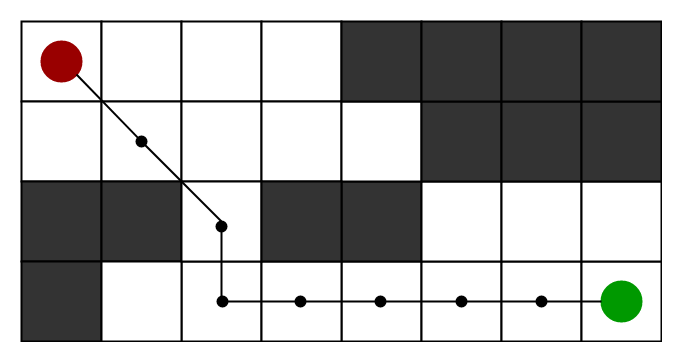
\includegraphics[width=0.7\linewidth]{a_-search-algorithm-1}
			\caption{Example of a grid with obstacles. Credit: \bref{https://www.geeksforgeeks.org/a-search-algorithm/}{geeksforgeeks.org}}
			\label{fig:a-search-algorithm-1}
		\end{figure}
		
		
	\end{flushleft}
\end{frame}




\myqrframe

\end{document}
